\documentclass[12pt]{article}
\usepackage{mathematics}

\begin{document}

\subsection*{1A}
\begin{mdframed}
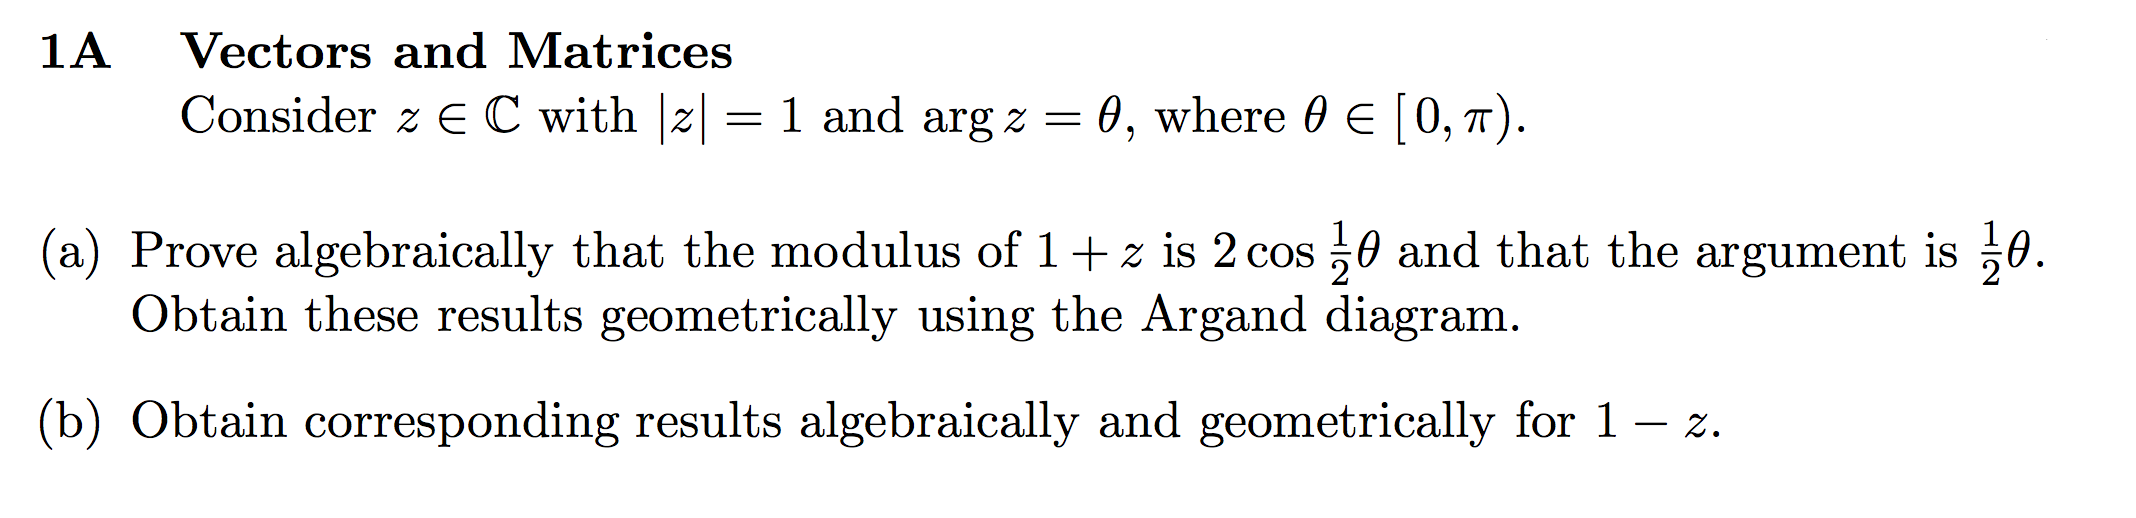
\includegraphics[width=400pt]{img/misc--cambridge-1a-2017-1-1A.png}
\end{mdframed}
\begin{proof}(Algebraic)\\
Note that
$\cos\theta = \cos^2\frac{1}{2}\theta - \sin^2\frac{1}{2}\theta = 2\cos^2\frac{1}{2}\theta - 1$.

We have $z = \cos\theta + i\sin\theta$ and therefore
\begin{align*}
  |1 + z|  &= \sqrt{(1 + \cos\theta)^2 + \sin^2\theta}
             = \sqrt{2(1 + \cos\theta)}
             = \sqrt{2\Big(1 + 2\cos^2\frac{1}{2}\theta - 1\Big)}
             = 2\cos\frac{1}{2}\theta\\
  |1 - z| &= \sqrt{(1 - \cos\theta)^2 + \sin^2\theta}
            = \sqrt{2(1 - \cos\theta)}
            = \sqrt{2(1 - (2\cos^2\frac{1}{2}\theta - 1))}
            = 2\sin\frac{1}{2}\theta.
\end{align*}
\end{proof}

\begin{proof}(Geometric)\\
  \begin{mdframed}
    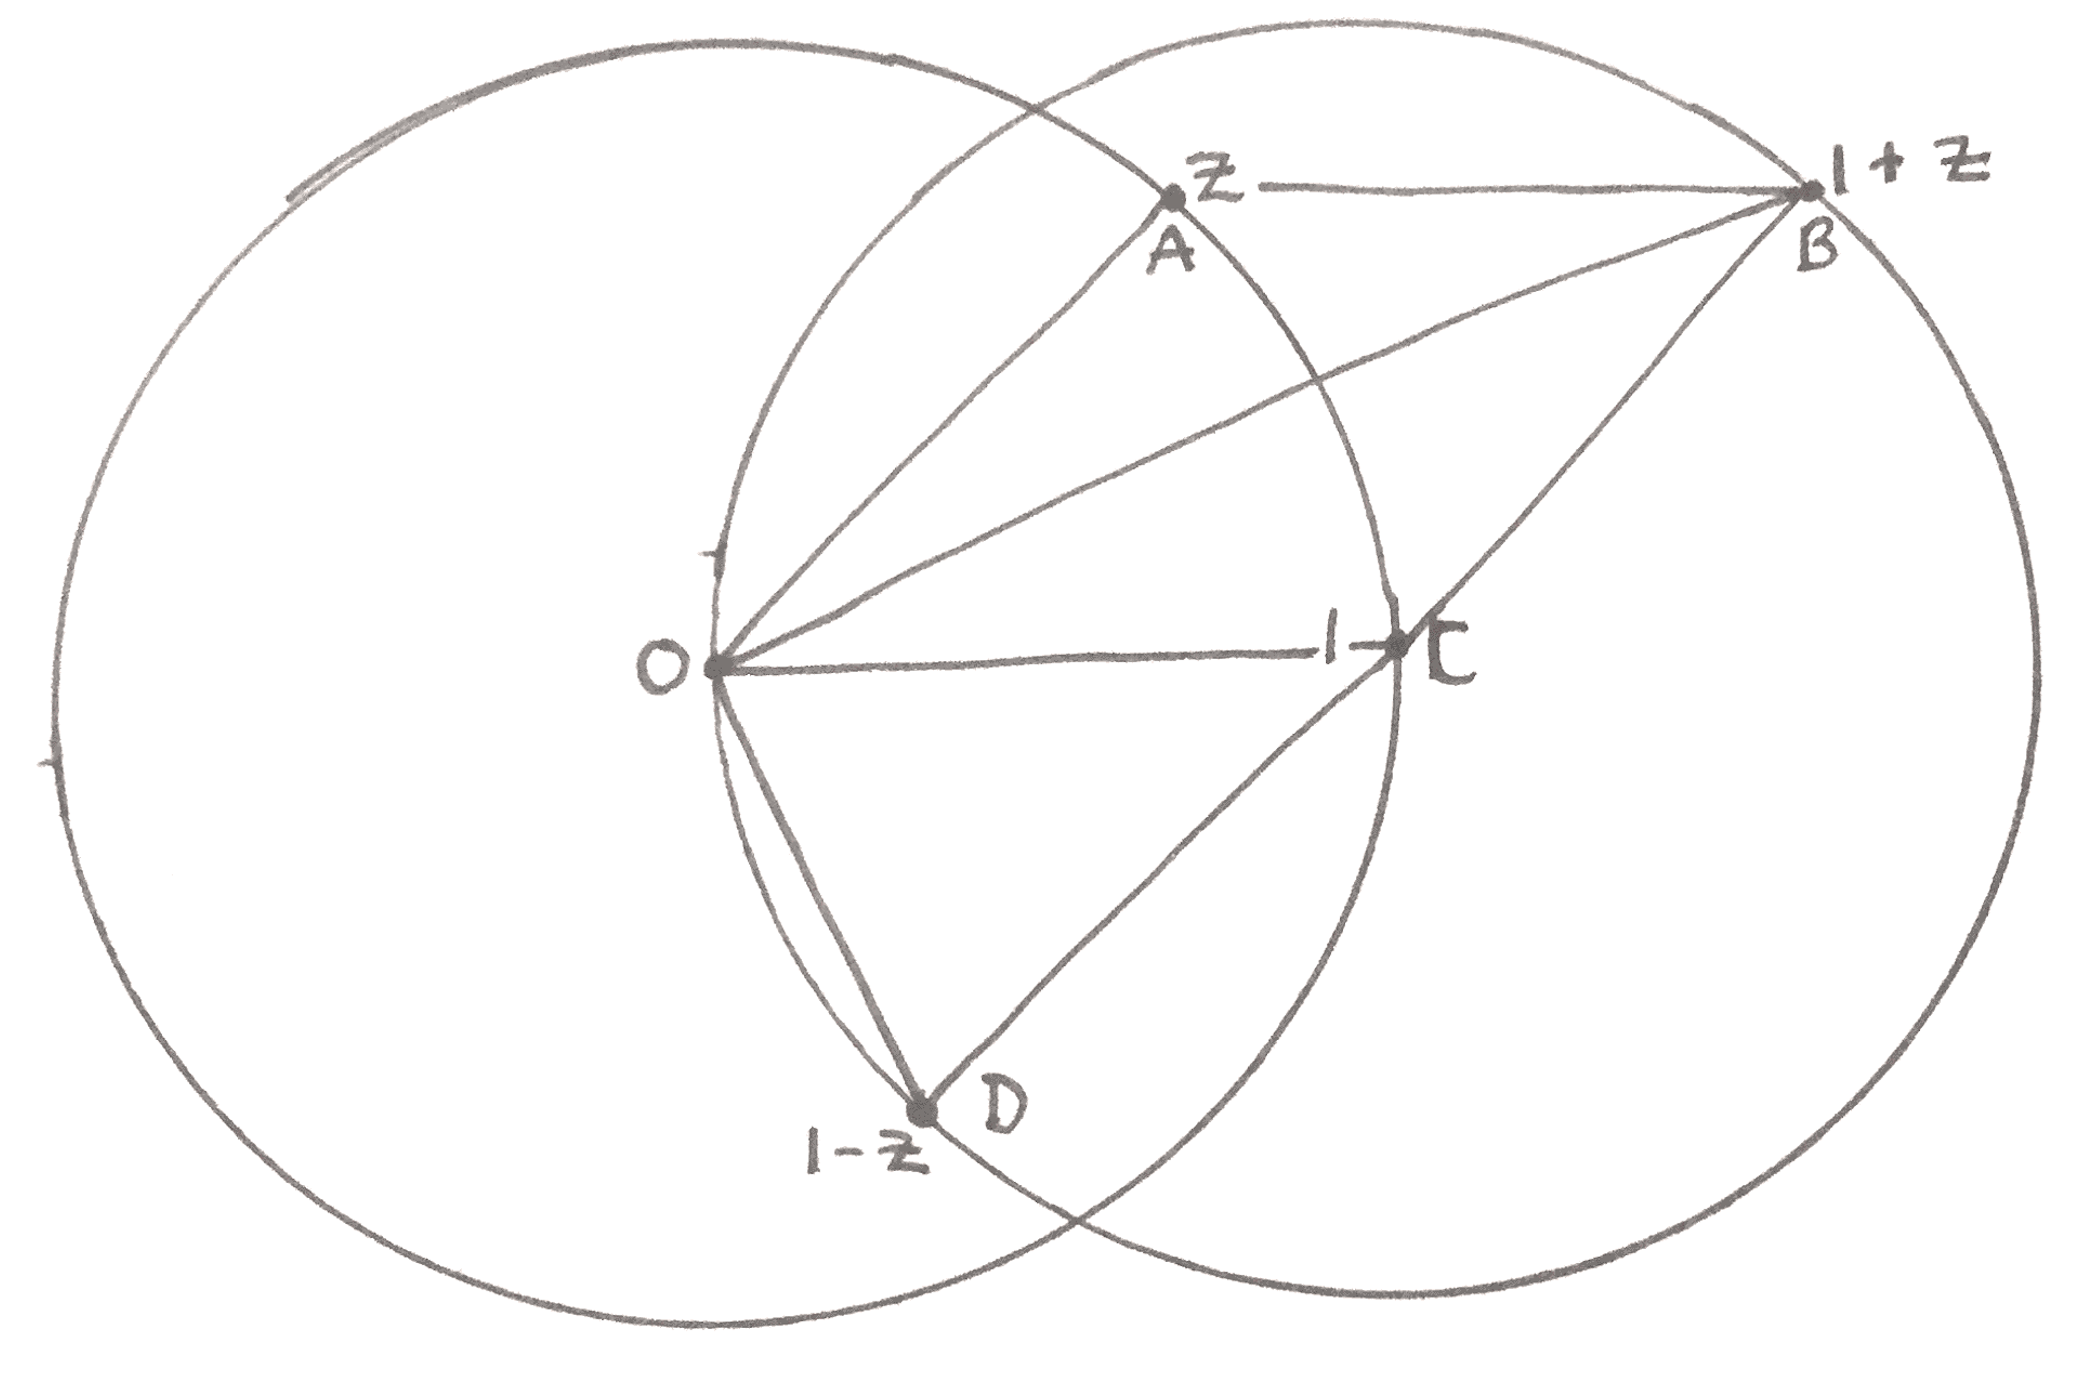
\includegraphics[width=300pt]{img/misc--cambridge-1a-2017-1-1A-diagram.png}
  \end{mdframed}
  $OABC$ is a rhombus, with sides of length 1 and $\angle AOC=\theta$. The diagonal $OB$ bisects
  $\angle AOC$, therefore $\angle OBC = \theta/2$. $\angle BOD$ is a right angle since it is formed
  from a triangle inscribed in a circle. Hypotenuse $BD$ has length 2, since $C$ is the centre of a
  second unit circle with radii $CB$ and $CD$. Therefore the length of $OB$ is
  $2\cos\frac{1}{2}\theta$ and the length of $OD$ is $2\sin\frac{1}{2}\theta$.
\end{proof}


\newpage
\subsection*{2C}
\begin{mdframed}
  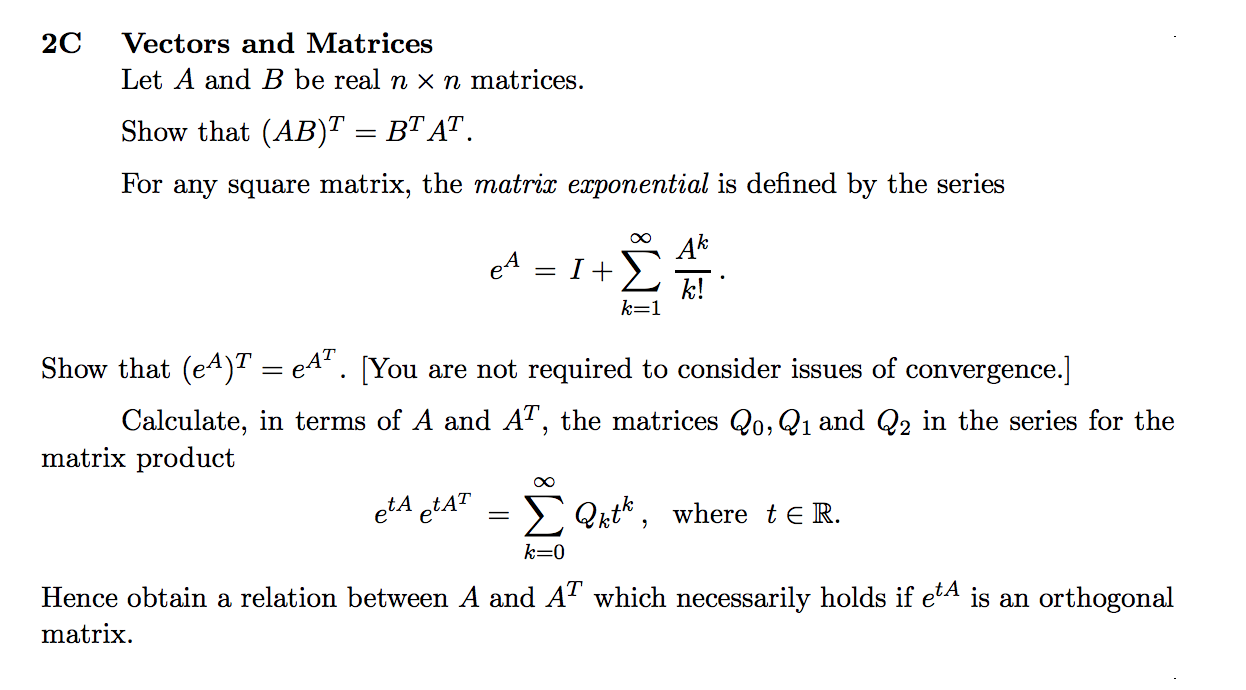
\includegraphics[width=400pt]{img/misc--cambridge-1a-2017-1-2c.png}
\end{mdframed}

\begin{claim*}
  $(AB)^T = B^TA^T$
\end{claim*}

\begin{proof}
  Let $i, j \in \{1, \ldots, n\}$. Then
  \begin{align*}
    \((AB)^T\)_{ij} = (AB)_{ji}
                   = \sum_{l=1}^n A_{jl}B_{li}
                   = \sum_{l=1}^n (A^T)_{lj}(B^T)_{il}
                   = (B^TA^T)_{ij}
  \end{align*}
\end{proof}

\begin{lemma*}
  $(A^k)^T = (A^T)^k$.
\end{lemma*}

\begin{proof}
  Note that $(A^m)^T(A^T)^n = (AA^{m-1})^T(A^T)^n = (A^{m-1})^T(A^T)^{n+1}$. By iterating this
  formal manipulation $k$ times, we have $(A^k)^T = (A^k)^T(A^T)^0 = (A^0)^T(A^T)^k = (A^T)^k$.
\end{proof}

\newpage
\begin{claim*}
  $(e^A)^T = e^{(A^T)}$
\end{claim*}

\begin{proof}
  Note that $(e^A)_{ij} := \sum_{k=0}^\infty \frac{(A^k)_{ij}}{k!}$, where $A^0 := I$ and
  $0! := 1$.  Therefore
  \begin{align*}
    \((e^A)^T\)_{ij} = \sum_{k=0}^\infty \frac{((A^k)^T)_{ij}}{k!}
                    = \sum_{k=0}^\infty \frac{((A^T)^k)_{ij}}{k!}
                    = \(e^{(A^T)}\)_{ij} .
  \end{align*}
\end{proof}

\begin{problem*}
  For $t \in \R$ we define matrices $Q_k$ such that $e^{tA}e^{tA^T} = \sum_{k=0}^\infty
  Q_kt^k$. Calculate $Q_0, Q_1, Q_2$.
\end{problem*}

\begin{proof}[Solution]~\\
  Note that
  \begin{align*}
    e^{tA}e^{tA^T}
    &=
      \(\sum_{k=0}^\infty\frac{(tA)^k}{k!}\)
      \(\sum_{k=0}^\infty \frac{(tA^T)^k}{k!}\)\\
    &=
      \(\sum_{k=0}^\infty\frac{t^k}{k!}A^k\)
      \(\sum_{k=0}^\infty \frac{t^k}{k!}(A^k)^T\).
  \end{align*}
  Therefore, by considering the coefficients of $t^0, t^1$ and $t^2$ in the expansion,
  \begin{align*}
    Q_0 &= I\\
    Q_1 &= A + A^T\\
    Q_2 &= AA^T + \frac{1}{2}(A^2 + (A^2)^T).
  \end{align*}

  If $e^{tA}$ is orthogonal, then
  $e^{tA}e^{tA^T} = e^{tA}e^{((tA)^T)} = e^{tA}(e^{tA})^T = e^{tA}(e^{tA})^\1 = I = \sum_{k=0}^\infty Q_kt^k$.

  Therefore $\sum_{k=1}^\infty Q_kt^k = 0$ for all $t$.

  Therefore $Q_k = 0$ for $k \in \{1, 2, \ldots\}$ \red{TODO: proof}.

  In particular, $Q_1 = 0$, therefore $A^T = -A$.

  As a check, we have $Q_2 = -A^2 + \frac{1}{2}(A^2 + (-A)^2) = 0$, as required.
\end{proof}

\newpage
\subsection*{3F}
\begin{mdframed}
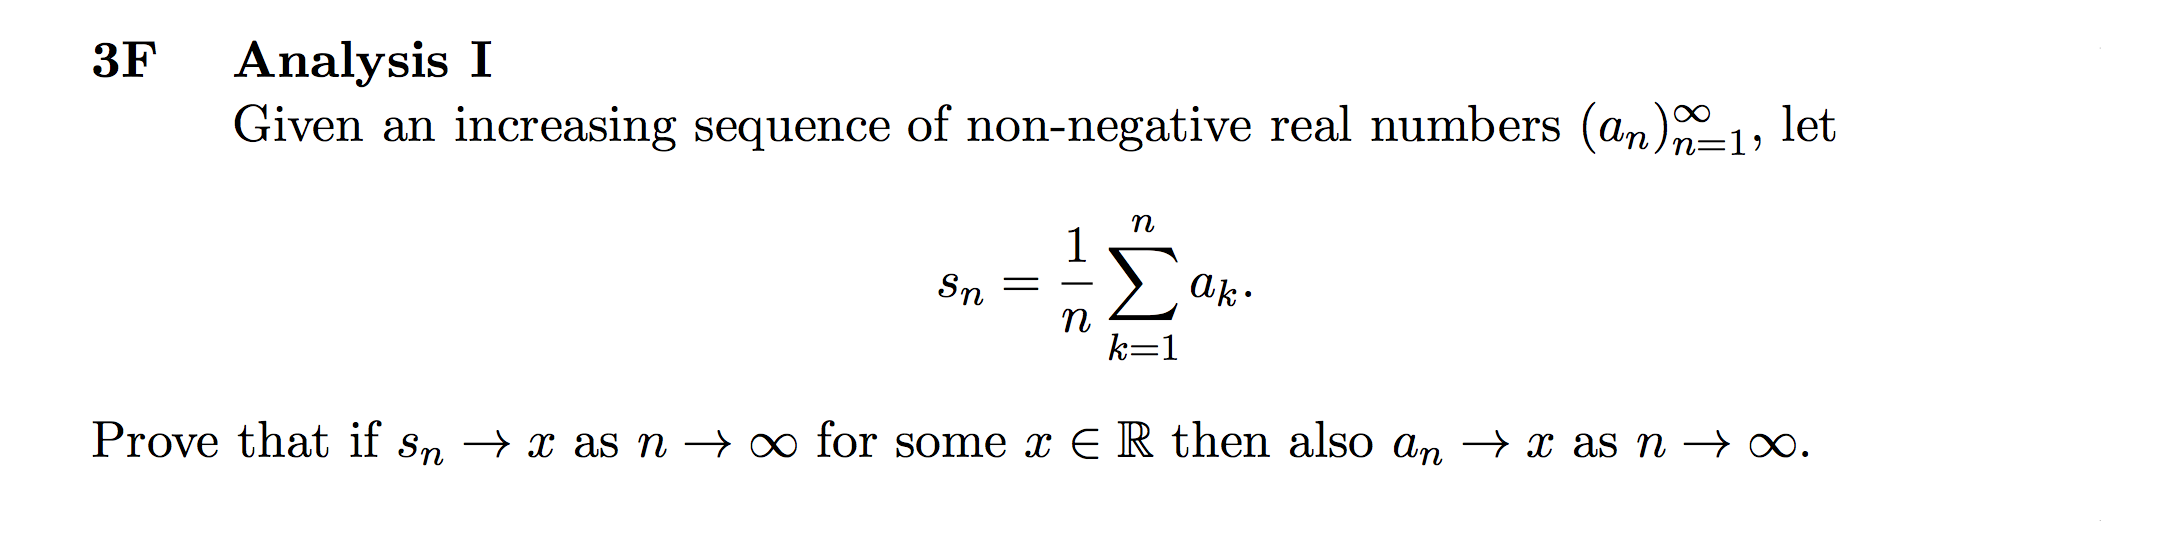
\includegraphics[width=400pt]{img/misc--cambridge-1a-2017-1-3f.png}
\end{mdframed}

\begin{proof}
  Assume that $s_n \to x$ as $n \to \infty$. We will show that $s_n \leq a_n \leq x$, for all $n$,
  therefore $a_n \to x$ as $n \to \infty$, as required.

  First note that $s_{n+1} = \frac{n}{n+1}s_n + \frac{1}{n+1}a_{n+1}$.
  % Note that $s_{n+1} = \frac{1}{n+1}\(\sum_{k=1}^na_k + a_{n+1}\) = \frac{n}{n+1}s_n + \frac{1}{n+1}a_{n+1}$.

  It's intuitively obvious that $s_n \leq a_n$ for all $n$. To prove this, note that it's true for
  $n = 1$; assume for induction that it's true for $n = k$. Then we have
  $s_{k+1} = \frac{k}{k+1}s_k + \frac{1}{k+1}a_{k+1} \leq \frac{k}{k+1}a_k + \frac{1}{k+1}a_{k+1}
  \leq a_{k+1}$, as required.

  Finally we show that $a_n \leq x$ for all $n$. Seeking a contradiction, assume that there exists
  $M$ such that $a_M > x$. Let $\epsilon = a_M - x > 0$, so that $a_n > x + \epsilon$ for $n > M$
  (see diagram). Then for $n > M$ we have
  \begin{align*}
    s_n &= \frac{1}{n}\sum_{k=1}^M a_k + \frac{1}{n}\sum_{k=M+1}^n a_k\\
        &> \frac{1}{n}\sum_{k=1}^M a_k + \frac{n - M}{n}(x + \epsilon).
  \end{align*}
  Therefore $\lim_{n\to\infty}s_n > x + \epsilon$ which is a contradiction, proving that
  $a_n \leq x$ for all $n$.
\begin{mdframed}
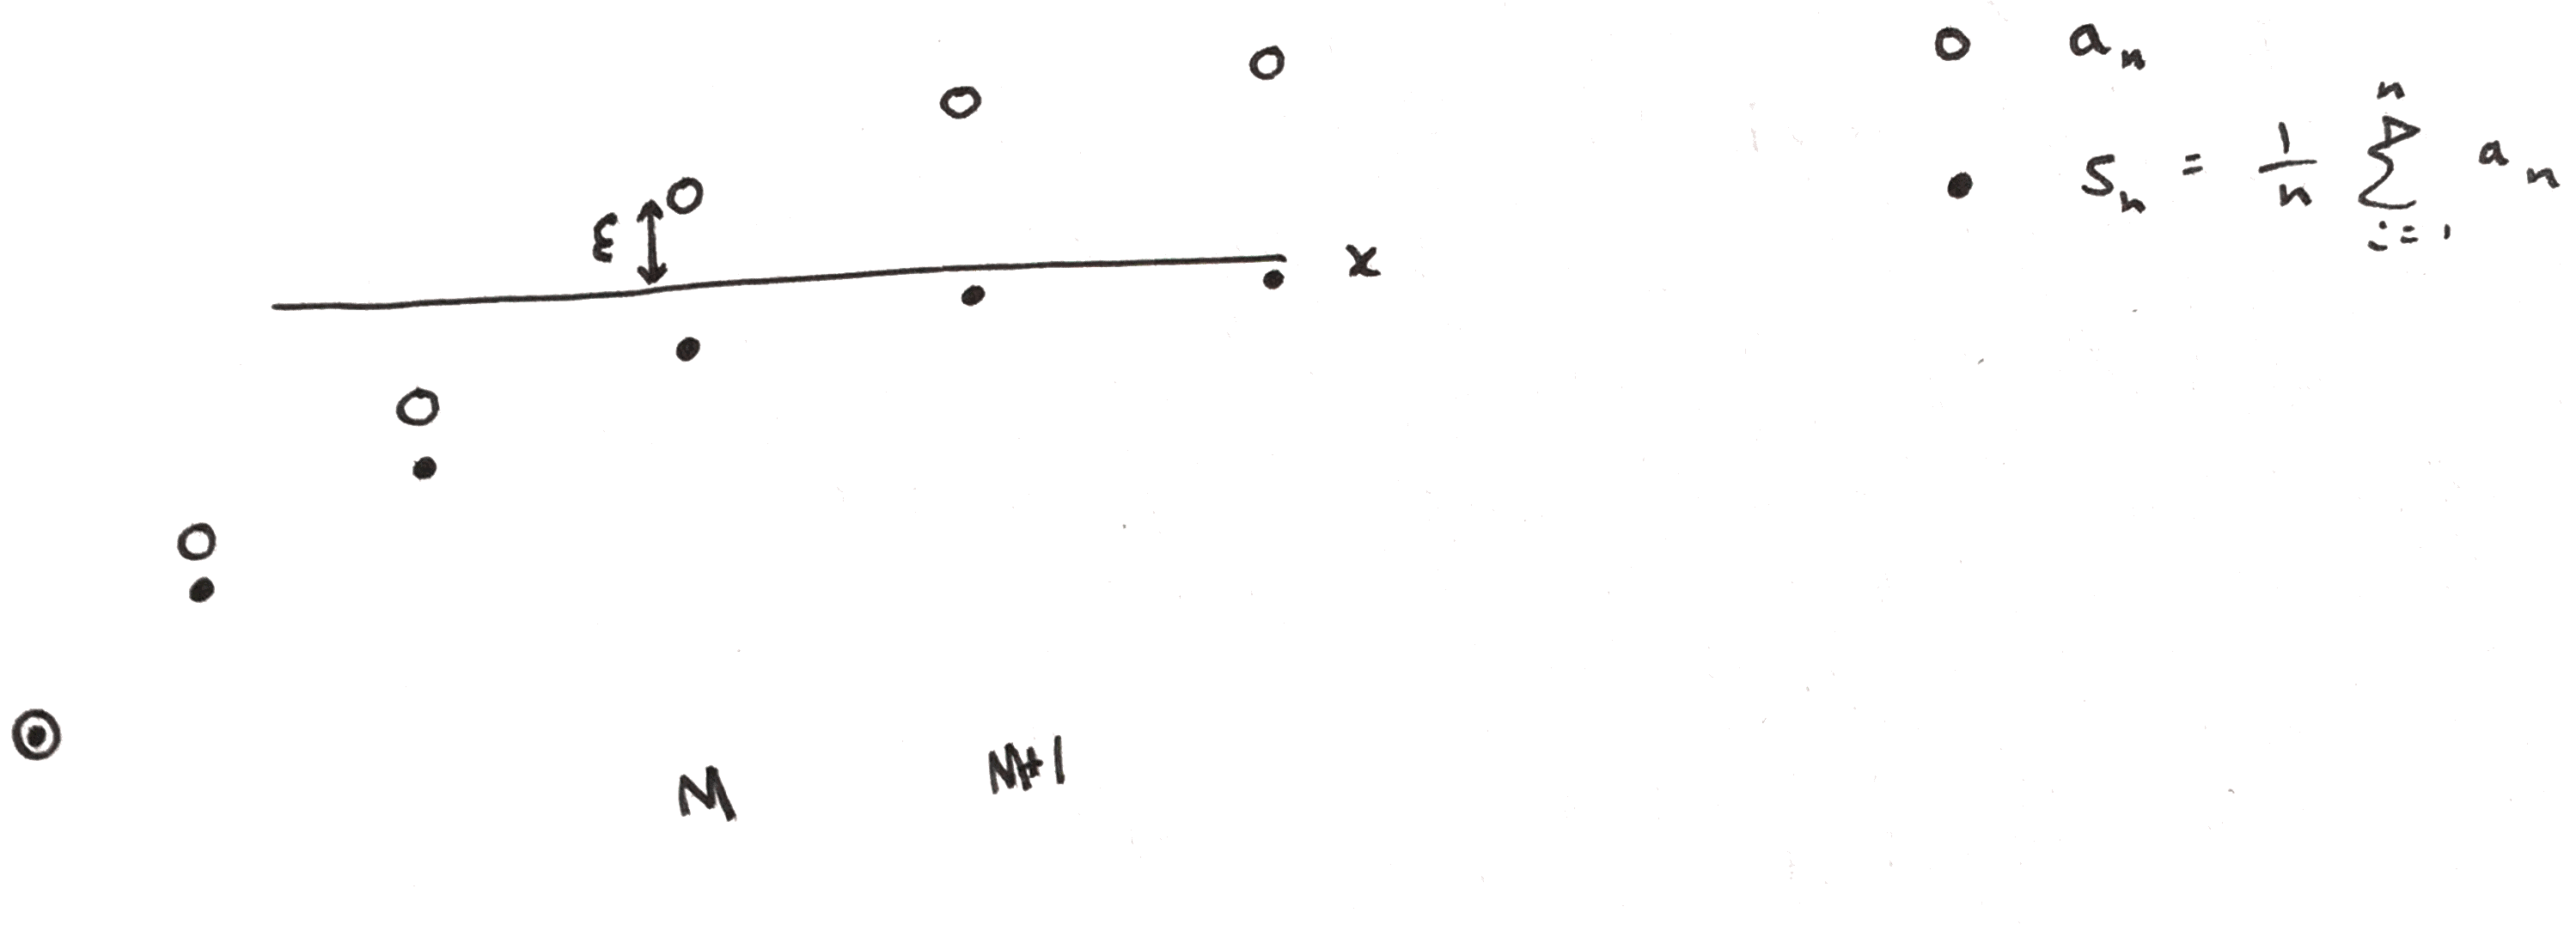
\includegraphics[width=400pt]{img/misc--cambridge-1a-2017-1-3f-diagram.png}
\end{mdframed}
\end{proof}



\begin{mdframed}
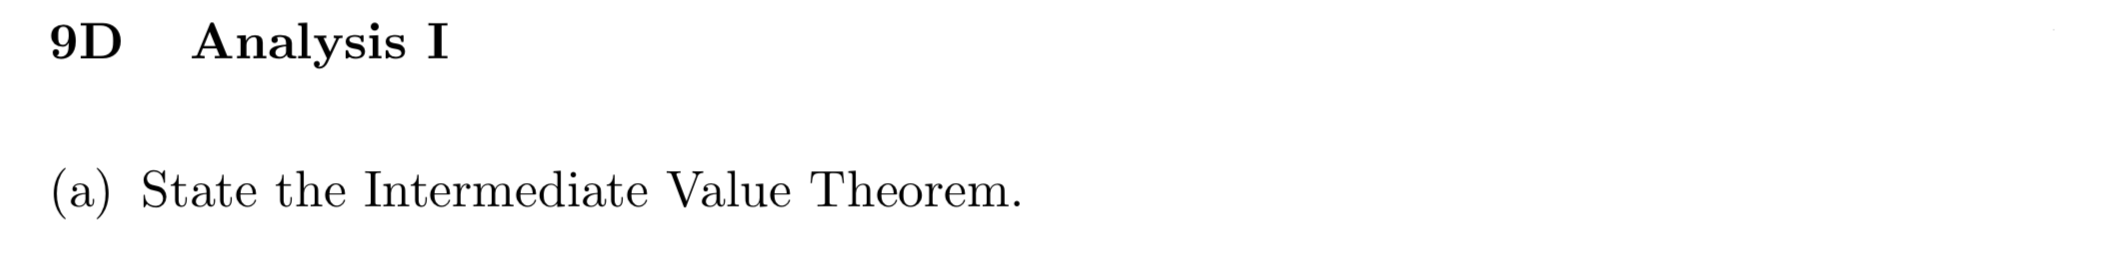
\includegraphics[width=400pt]{img/misc--cambridge-1a-2017-1-9D-1.png}
\end{mdframed}

\begin{definition*}[Completeness of reals I]
  For an ordered set: every non-empty subset that's bounded above has a least upper bound.
\end{definition*}


\begin{definition*}[Completeness of reals II]
  Every Cauchy sequence converges (to a value in the set).
\end{definition*}


\begin{theorem*}[Intermediate Value Theorem]~\\
  Let $a, b \in \R$, and $f:[a, b] \to \R$ be continuous. Let $u$ lie strictly between $f(a)$ and
  $f(b)$. Then there exists $c \in (a, b)$ such that $f(c) = u$.
\end{theorem*}

\begin{remark*}
  The proof first uses completeness of $\R$ (every non-empty subset with an upper bound has a least
  upper bound / supremum) to establish that a supremum $c$ exists. Then it uses continuity of $f$
  at that supremum to show $f(c) = u$.
\end{remark*}

\begin{proof}
  Define $S = \{x \in [a, b] ~|~ f(x) < u\}$.

  Note that $a \in S$ so $S \neq \emptyset$, and $S$ bounded above by $b$ so $\sup S$ exists, by
  completeness of the reals. Let $c = \sup S$. We claim that $f(c) = u$.

  To prove this, we will show that for all $\epsilon > 0$, we have
  $u - \epsilon < f(c) < u + \epsilon$.

  Fix an $\epsilon > 0$.

  Since $f$ is continuous at $c$, we have that there exists $\delta > 0$ such that
  \begin{align*}
    |x - c| < \delta \implies |f(x) - f(c)| < \epsilon.
  \end{align*}

  First consider a point $a^* \in (c - \delta, c)$. We have
  \begin{align*}
    f(a^*) < u                                    ~~~~~~~&\text{since $a^* \in S$}\\
    f(c) - \epsilon < f(a^*) < f(c) + \epsilon    ~~~~~~~&\text{by continuity of $f$ at $c$},
  \end{align*}
  therefore $f(c) < u + \epsilon$.

  Next consider a point $a^{**} \in (c, c + \delta)$. We have
  \begin{align*}
    f(a^{**}) > u                                  ~~~~~~~&\text{since $a^{**} \notin S$}\\
    f(c) - \epsilon < f(a^{**}) < f(c) + \epsilon  ~~~~~~~&\text{by continuity of $f$ at $c$},
  \end{align*}
  therefore $f(c) > u - \epsilon$.

  Therefore $u - \epsilon < f(c) < u + \epsilon$ as required.
\end{proof}

\begin{mdframed}
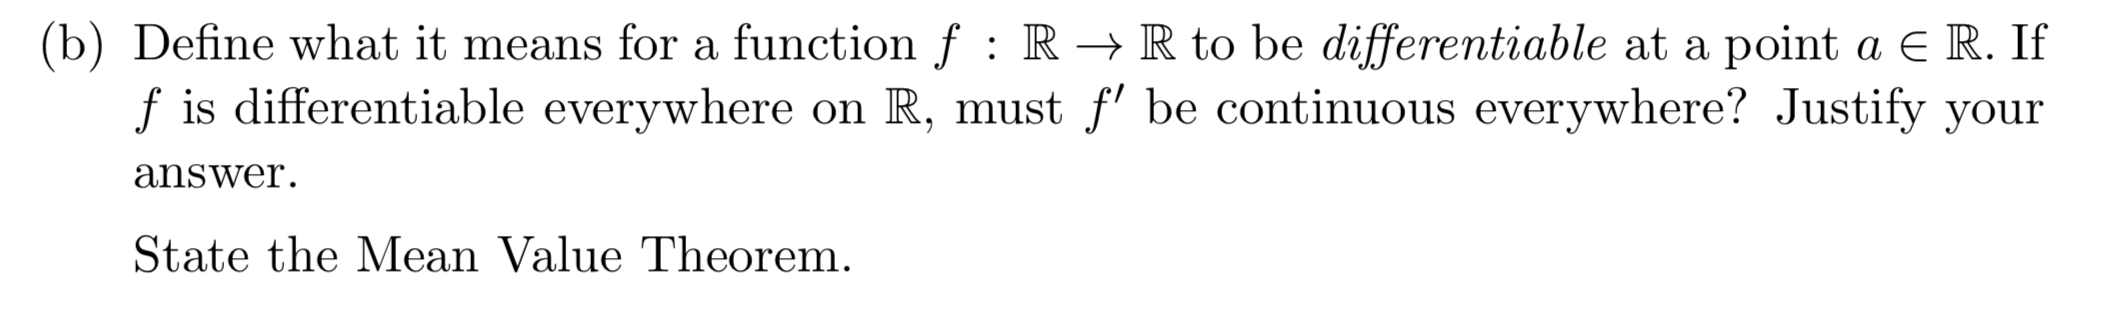
\includegraphics[width=400pt]{img/misc--cambridge-1a-2017-1-9D-2.png}
\end{mdframed}

\begin{definition*}
  Let $f: \R \to \R$ and $a \in \R$. If the limits
  \begin{align*}
    \lim_{x \to a^+} \frac{f(x) - f(a)}{x - a}\\
    \lim_{x \to a^-} \frac{f(x) - f(a)}{x - a}
  \end{align*}
  both exist and are equal then $f$ is differentiable at $a$.
\end{definition*}


\begin{definition*}
  Let $f: \R \to \R$ and $a \in \R$. If the limit
  \begin{align*}
    \lim_{x \to a} \frac{f(x) - f(a)}{x - a}
  \end{align*}
  exists then $f$ is differentiable at $a$.
\end{definition*}




\begin{theorem*}
  $f$ differentiable everywhere on $\R$ does not imply $f'$ continuous everywhere on $\R$.
\end{theorem*}

\begin{proof}
We exhibit a counterexample: a function that is differentiable everywhere on $\R$ but $f'$ is not
continuous everywhere.

Consider
\begin{align*}
  f(x) :=
  \begin{cases}
    x^2\sin(\frac{1}{x}),~~~~~~~&x \neq 0\\
    0                    ~~~~~~~&x = 0,
  \end{cases}
\end{align*}
the derivative of which is\footnote{The derivative at $x = 0$ is
  $\lim_{x\to 0}\frac{x^2\sin\(\frac{1}{x}\) - 0}{x - 0} = \lim_{x\to 0}x\sin\(\frac{1}{x}\)$. Note
  that $x\sin\(\frac{1}{x}\)$ is bounded above and below by $x$ and $-x$. Since these both have a
  limit of 0 at $x=0$, then so must $x\sin\(\frac{1}{x}\)$.  }
\begin{align*}
  f'(x) =
  \begin{cases}
    2x\sin(\frac{1}{x}) -\cos(\frac{1}{x}) ~~~~~~~ &x \neq 0\\
    0                                      ~~~~~~~ &x = 0.
  \end{cases}
\end{align*}

Note that $f(x)$ is continuous since it is differentiable. But $f'(x)$ is not continuous at 0,
since close to 0, arbitrarily small changes to $x$ will cause $\cos\(\frac{1}{x}\)$ to vary between
-1 and 1. To prove this, note that
\begin{align*}
  \lim_{x\to 0} f'(x) = 2\lim_{x\to 0} x\sin\(\frac{1}{x}\) - \lim_{x\to 0}\cos\(\frac{1}{x}\)
                     = - \lim_{x\to 0}\cos\(\frac{1}{x}\).
\end{align*}
Fix $0 < \epsilon \leq 1$ and suppose that there exists $\delta > 0$ such that
$|x| < \delta \implies |\cos\(\frac{1}{x}\)| < \epsilon$. But now define
$k = \lceil\frac{1}{\delta}\rceil$ and consider $x = \frac{1}{2k\pi}$. We have $|x| < \delta$ but
$\cos\(\frac{1}{x}\) = 1 \geq \epsilon$, a contradiction proving that
$\lim_{x\to 0}\cos\(\frac{1}{x}\)$ does not exist.
\end{proof}


\begin{theorem*}[Mean-value theorem]
  Let $a, b \in \R$ with $b > a$, and $f:[a,b] \to \R$ be continuous on $[a, b]$ and differentiable
  on $(a, b)$. Then there exists $x \in (a, b)$ such that $f'(x) = \frac{f(b) - f(a)}{(b - a)}$.
\end{theorem*}


\begin{mdframed}
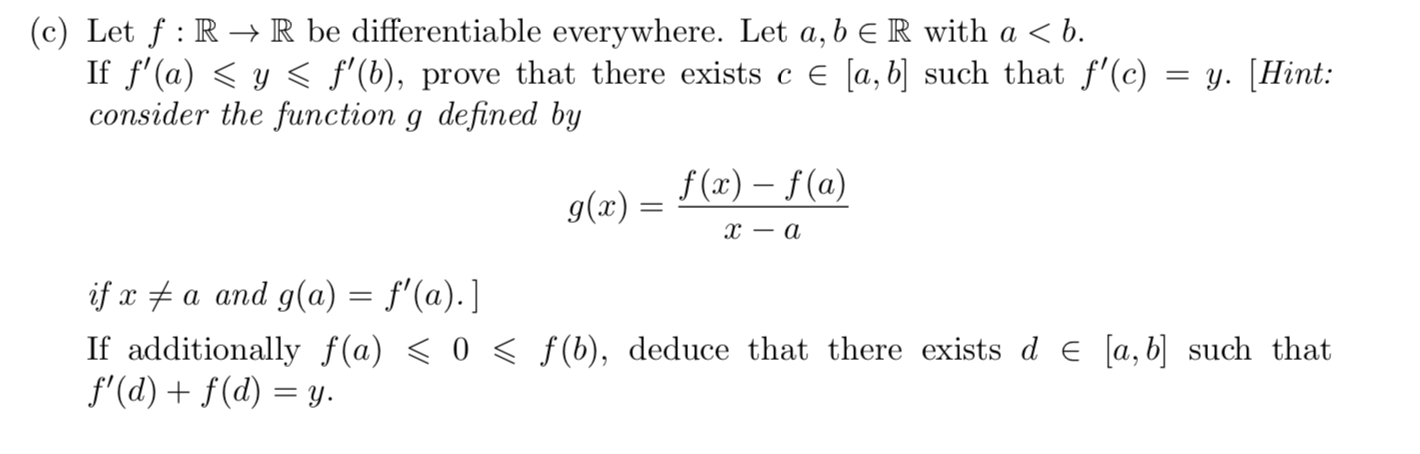
\includegraphics[width=400pt]{img/misc--cambridge-1a-2017-1-9D-3.png}
\end{mdframed}


\begin{theorem*}
  Let $f: \R \to \R$ be differentiable. Let $a, b \in \R$ with $a < b$. If
  $f'(a) \leq y \leq f'(b)$, then there exists $c \in [a, b]$ such that $f'(c) = y$.
\end{theorem*}

\begin{remark*}
  This does not follow from the Intermediate Value Theorem, since that theorem requires continuity:
  the derivative of a continuous function may not itself be continuous.
\end{remark*}

\begin{proof}
  Define
  \begin{align*}
    g(x) :=
    \begin{cases}
      \frac{f(x) - f(a)}{x - a} ~~~~~~~ &x \neq a\\
      f'(a) ~~~~~~~ &x = a.
    \end{cases}
  \end{align*}

  {\bf Scratch}\\
  Is $g$ continuous? Suppose it is.

  We know $f'(a) \in \Im g$.

  Note that, by the Mean Value Theorem, there exists $x \in (a, b)$ such that $f'(x) = g(b)$.


\end{proof}

\newpage
\begin{mdframed}
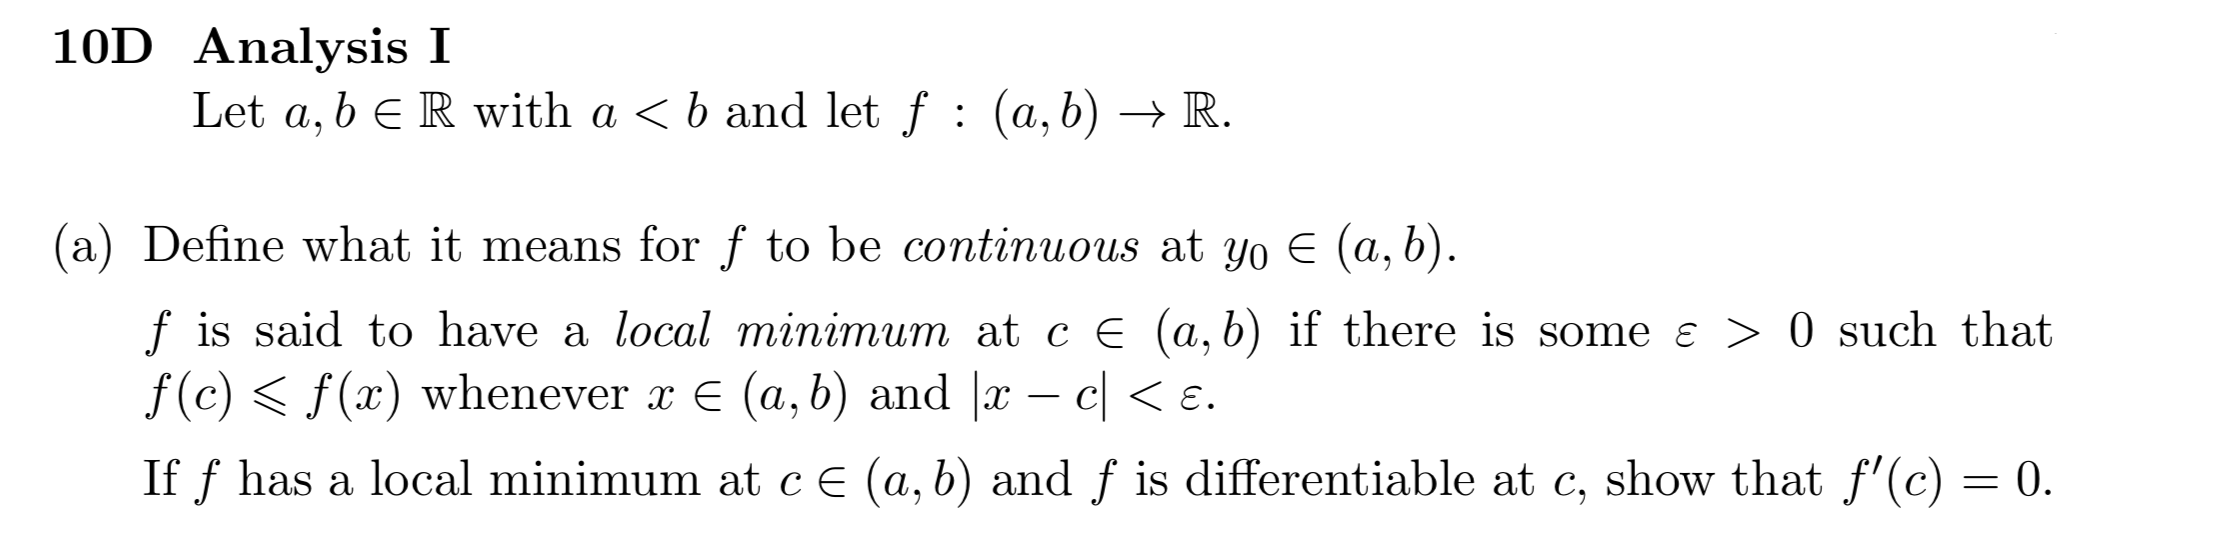
\includegraphics[width=400pt]{img/misc--cambridge-1a-10D-a.png}
\end{mdframed}

$f$ is continuous at $x_0 \in (a, b)$ iff $\lim_{x\to x_0} f(x) = f(x_0)$.

We know:

\begin{enumerate}
\item The limit $L = f'(c) := \lim_{x\to c} \frac{f(x) - f(c)}{x - c}$ exists.
\item For every $\epsilon > 0$ there exists $\delta > 0$ such that
  $|x - c| < \delta \implies \Big|\frac{f(x) - f(c)}{x - c} - L\Big| < \epsilon$.
\item $f$ is continuous at $c$: $\lim_{x\to c}f(x) = f(c)$.
\item There exists $\delta > 0$ such that $|x - c| < \delta \implies f(c) \leq f(x)$.
\end{enumerate}

We want:
\begin{align*}
  L = 0.
\end{align*}


\newpage

\begin{mdframed}
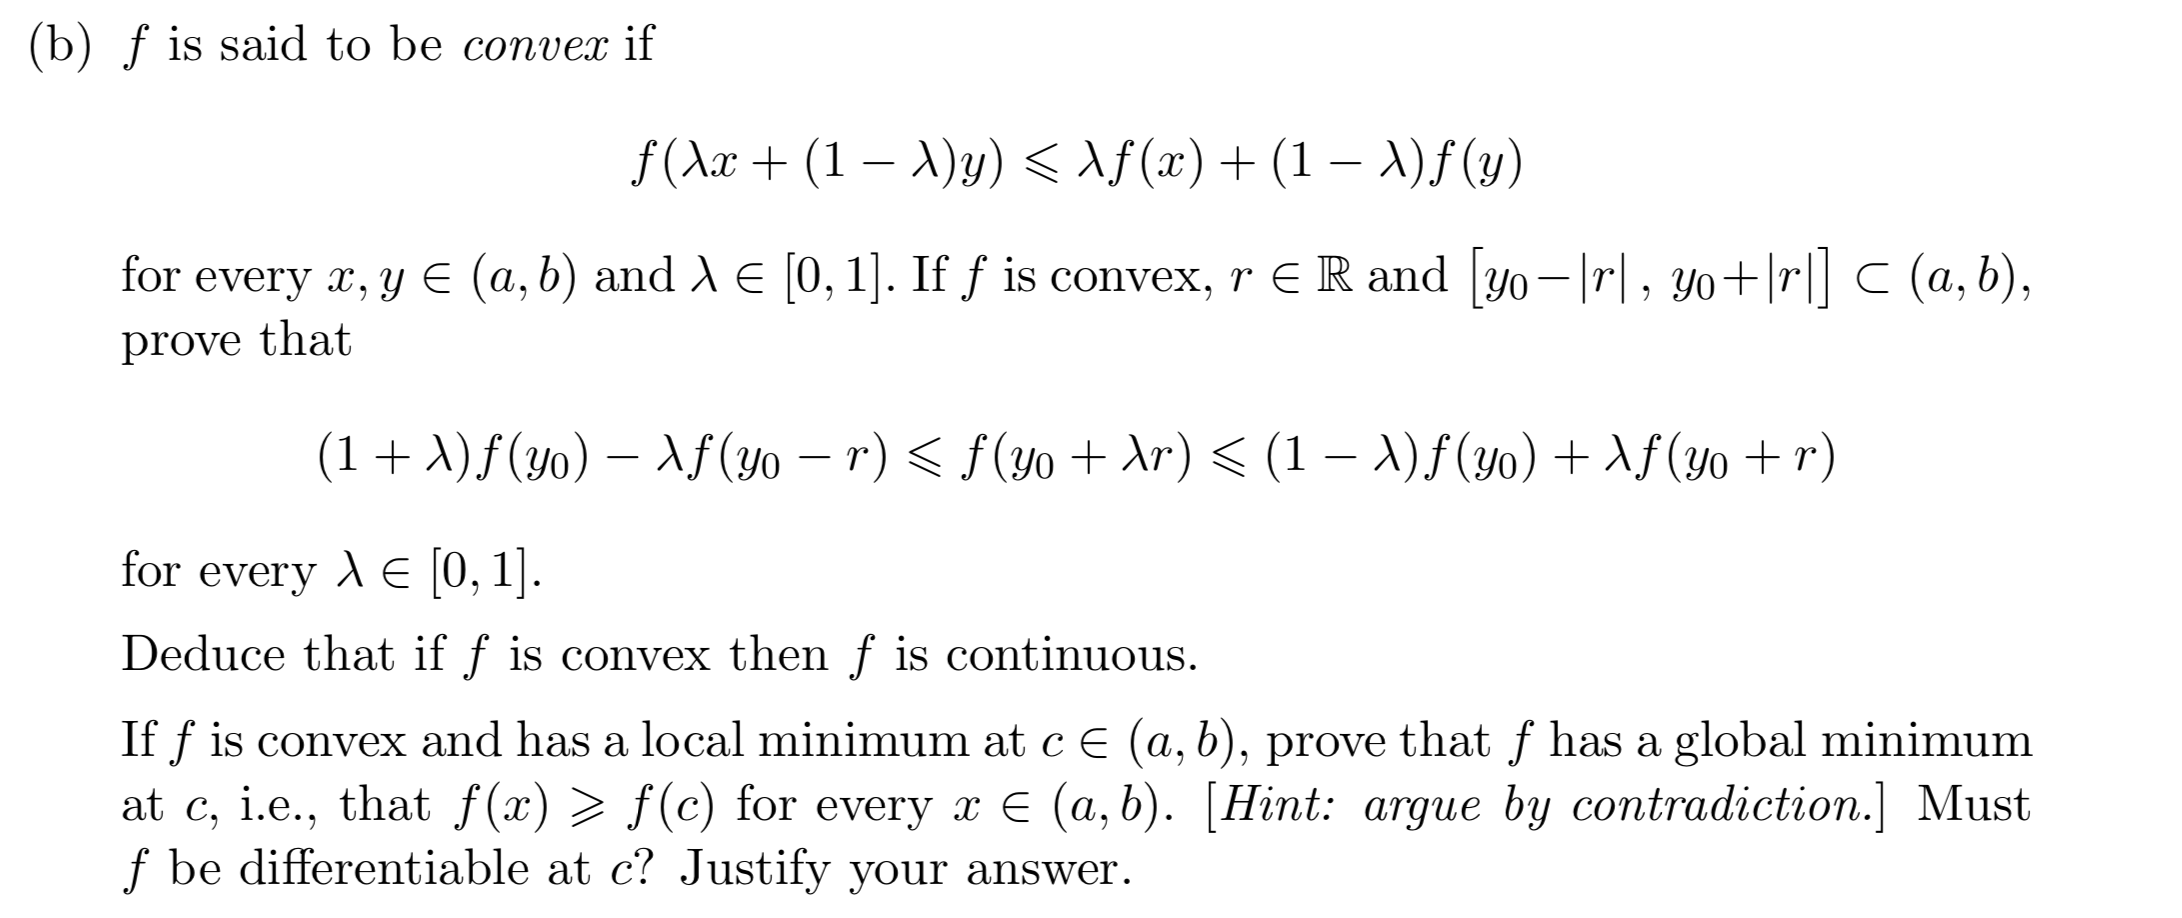
\includegraphics[width=400pt]{img/misc--cambridge-1a-10D-b.png}
\end{mdframed}

\end{document}
